\documentclass{article}
\usepackage{fullpage}

%load needed packages
\usepackage{graphicx}
\usepackage{array}
\usepackage{booktabs}
\usepackage[utf8]{inputenc}
\usepackage[T1]{fontenc}

\usepackage[spanish]{babel} % Paquete para el idioma español
\usepackage{float}  % Necesario para [H]
\usepackage{listings}
\usepackage{xcolor}

\definecolor{codegreen}{HTML}{5AB2FF}
\definecolor{morado}{HTML}{AD88C6}
\definecolor{BG}{HTML}{EEEEEE}
\definecolor{azul}{HTML}{4D869C}
\definecolor{sqlblue}{HTML}{FF8C00} % Color para las palabras clave SQL

% Estilo para DDL
\lstdefinestyle{ddlstyle}{
	language=SQL,
	backgroundcolor=\color{BG},
	commentstyle=\color{codegreen},
	basicstyle=\ttfamily\small,
	keywordstyle=\color{azul},
	stringstyle=\color{morado},
	showstringspaces=false,
	breaklines=true,
	frame=shadowbox,
	numbers=left,
	numberstyle=\tiny\color{gray},
	captionpos=b,
}

% Estilo para SQL
\lstdefinestyle{sqlstyle}{
	language=SQL,
	backgroundcolor=\color{BG},
	commentstyle=\color{codegreen},
	basicstyle=\ttfamily\small,
	keywordstyle=\color{sqlblue}, % Color diferente para palabras clave SQL
	stringstyle=\color{morado},
	showstringspaces=false,
	breaklines=true,
	frame=shadowbox,
	numbers=left,
	numberstyle=\tiny\color{gray},
	captionpos=b,
}

\begin{document}



% Portada
\begin{titlepage}
	\centering
	\vspace*{3cm}
	
	% Título destacado
	{\Huge \textbf{Practica 1: Bases De Datos Relacionales}\\[0.5cm]}
	
	% Espacio y logotipo (si lo tienes, por ejemplo el logo de tu universidad)
	\vspace{2cm}
	
\includegraphics[width=0.3\textwidth]{images/uma_logo.jpg}\\[1cm]
	
	% Nombre del autor
	{\LARGE \textbf{Alejandro Silva Rodríguez}\\[0.5cm]}
	{\LARGE \textbf{Marta Cuevas Rodríguez}\\[0.5cm]}
	{\large \textit{Almacenes De Datos}\\
		Universidad de Málaga\\
		}
	
	\vfill
	
	% Fecha en la parte inferior de la página
	{\large Septiembre 2024}
\end{titlepage}

% indice
\tableofcontents

\newpage

\section{Introducción}

En esta práctica, se diseñará y creará una base de datos para gestionar información sobre parques naturales en Andalucía y la liga española de fútbol de primera división. El objetivo es elaborar un modelo entidad-relación y un modelo relacional que muestren las características y relaciones de las entidades involucradas, utilizando herramientas de diseño de bases de datos.

Además, se generará el DDL (Data Definition Language) para SQL Server, que permitirá crear la base de datos y las tablas necesarias. Se incluirán datos sobre los parques naturales, su gestión y las especies que los habitan, así como información sobre los equipos de fútbol, sus jugadores y los partidos.

Este ejercicio ayudará a aplicar los conceptos de bases de datos y ofrecerá una experiencia práctica en el uso de herramientas y lenguajes de consulta.



\section{Parques Naturales}

En esta sección se explicara como se diseñó e implementó la base de datos de parques naturales y las consultas sobre la misma.

\subsection{Requisitos De Datos}

La Junta de Andalucía desea mantener la información sobre los parques naturales que hay en su comunidad autónoma. En particular sería necesario conocer el nombre del parque (que es único), su teléfono, dirección administrativa, una dirección web, un correo electrónico, su fecha de declaración como parque natural, la extensión (en hectáreas) de cada zona protegida, las especies animales que contiene, la población estimada de cada una de ellas y la dirección gestora del parque. Esta dirección gestora del parque está coordinada por un presidente y un número no determinado de consejeros. De todos estos miembros de la dirección gestora se desea conocer el DNI, nombre, fecha de nacimiento, dirección y teléfono de cada uno de ellos. Cada persona puede ser a lo sumo consejero en un parque y presidente de otro. De las especies guardamos su nombre científico y el común (ambos son únicos), el número de años de vida media. 
\\

Con objeto de poder determinar el estado de salud del parque necesitamos información sobre la interacción del hombre con el entorno. Para ello se almacenan datos sobre los municipios donde está ubicado el parque: número de municipios que abarca, nombre de cada uno de ellos, enlace a su web, fichero con la foto de su escudo, partido que gobierna en la alcaldía, número de habitantes y gasto de agua medio por habitante. 
\\

Las especies tienen una extensión (en hectáreas) necesaria para desarrollarse en libertad, dato que aparece en los estudios generales sobre cada especie. Sin embargo, el dato de si la especie está superpoblada en cada parque se guardará explícitamente, porque puede depender de factores como si el parque es montañoso, si tiene acuíferos, etc y por tanto precisa de la opinión última de un experto. Tenga en cuenta que cada municipio abarca a lo sumo un sólo parque. 

\newpage
\subsection{Diseño Lógico}

Para crear el diseño lógico de la base de datos en Oracle Datamodeler \cite{oracle2024} empezaremos representando las figuras más relevantes como entidades, entre ellas encontramos a especie animal, municipio, parque natural y persona (figura \ref{fig:p_logico}). Cada entidad tendrá atributos que solo pertenecen a ella y no se relacionan con ninguna entidad más excepto del atributo numero de municipios que abarca de un parque natural, tendrá que ir actualizandose mediante un trigger cada vez que se le añade o elimina una relación municipio.Tambien tendremos una entidad intermedia entre especie animal y parque natural que almacenará la relacion entre estas y los atributos extensión, población estimada y is\_superpoblado (booleano).
\\

Por ultimo, tenemos relaciones entre parque natural y municipio y dos entre parque natural y persona. Una relación 1:N representará los consejeros del parque natural y otra 1:1 representara el presidente del parque.

\begin{figure}[H]
	\centering
	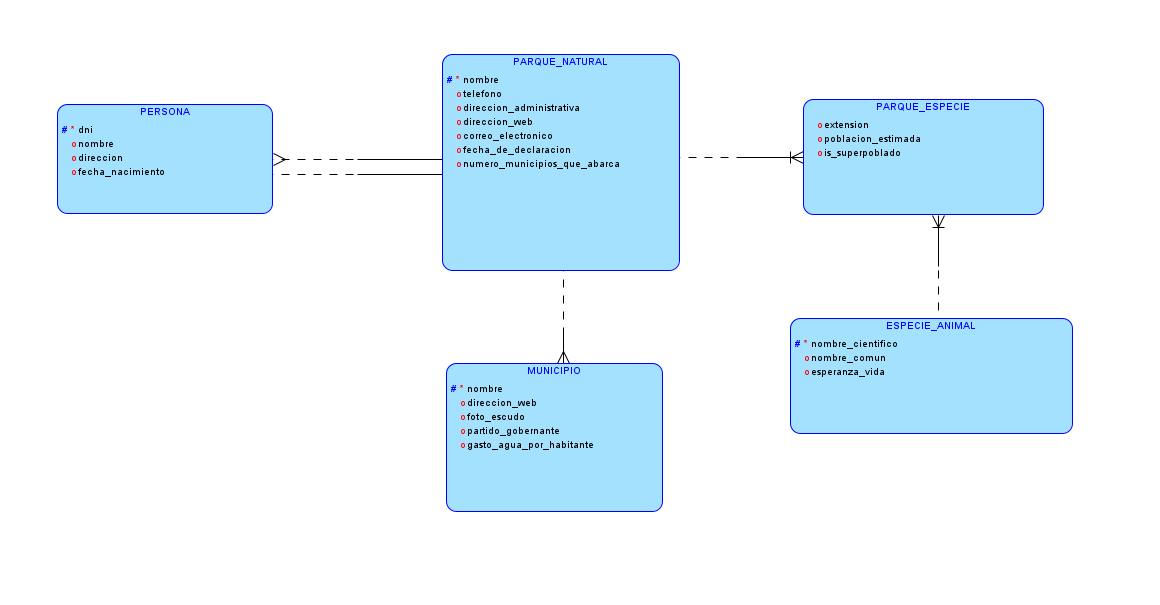
\includegraphics[width=\textwidth]{images/diagrama_logico_parques_naturales.png}
	\caption{Diagrama Lógico De Parques Naturales}
	\label{fig:p_logico}
\end{figure}

\newpage

\subsection{Diseño Entidad Relación}

En el diseño entidad relación tenemos que tener en cuenta que las claves y restricciones están donde se necesitan para poder hacer consultas en la base de datos. Observamos (figura \ref{fig:p_relacional}) que parque natural tiene una clave foranea dni que representa al unico presidente de esta entidad, mientras que persona tiene una clave foranea nombre de parque natural que relaciona a los consejeros con esta. Municipio obtiene la clave foranea de parque natural debido a su particion en la parte N de la relación. La entidad intermedia de especie animal y parque natural obtiene sus dos claves foraneas que pasan a ser su clave principal.

\begin{figure}[H]
	\centering
	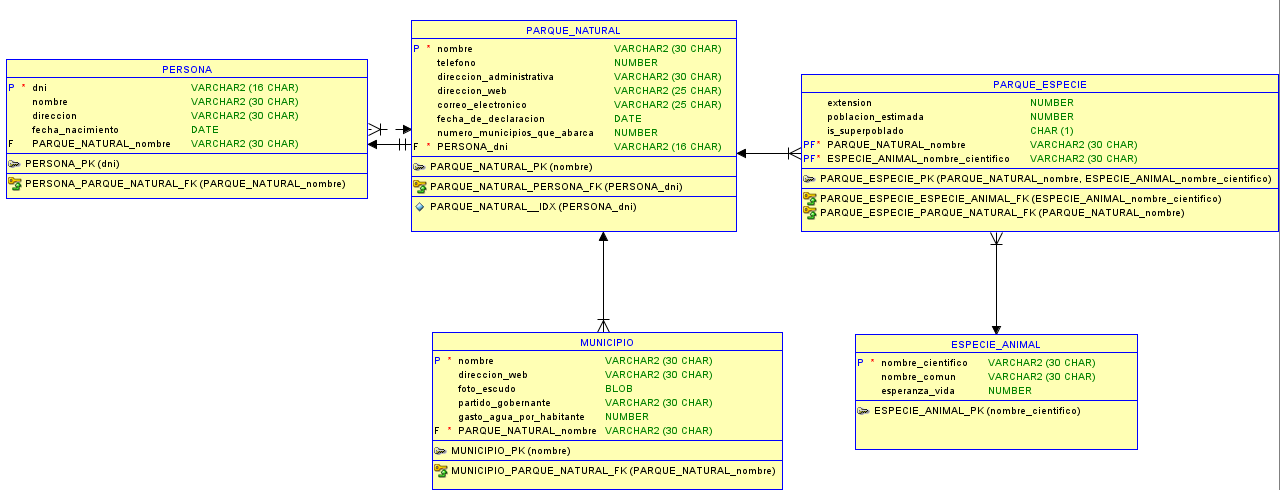
\includegraphics[width=\textwidth]{images/diagrama_relacional_parques_naturales.png}
	\caption{Diagrama Relacional De Parques Naturales}
	\label{fig:p_relacional}
\end{figure}

\subsection{Implementación}

En la implementación de la base de datos generaremos el ddl (data definition languaje) de la base de datos e insertaremos tuplas en la misma. En el listing \ref{fig:p_ddl} encontramos una pequeña parte del mismo donde se crea la tabla de especie animal. Esto se ejecutará en Microsoft SQL Server \cite{sqlserver2022} donde se alojará la base de datos.
\begin{lstlisting}[style=ddlstyle, label=fig:p_ddl,caption=Definicion De Datos De Parques Naturales]
	
	CREATE TABLE ESPECIE_ANIMAL 
	(
	nombre_cientifico VARCHAR (30) NOT NULL , 
	nombre_comun VARCHAR (30) , 
	esperanza_vida NUMERIC (28) 
	)
	GO
	
	ALTER TABLE ESPECIE_ANIMAL ADD CONSTRAINT ESPECIE_ANIMAL_PK PRIMARY KEY CLUSTERED (nombre_cientifico)
	WITH (
	ALLOW_PAGE_LOCKS = ON , 
	ALLOW_ROW_LOCKS = ON )
	GO
	
	
\end{lstlisting}
\newpage

En el listing \ref{fig:p_insert} se observan ejemplos de las inserciones que se hacen sobre la base de datos y el trigger que añadimos para la actualización del número de municipios. Es crucial seguir un orden logico a la hora de la inserción ya que algunas entidades dependen de otras.
\begin{lstlisting}[style=sqlstyle, label=fig:p_insert,caption=Carga de datos]
	-- Insertar especies animales
	INSERT INTO ESPECIE_ANIMAL (nombre_cientifico, nombre_comun, esperanza_vida) VALUES
	('Ursus arctos', 'Oso pardo', 25),
	-- Insertar personas (presidentes) - un presidente por parque natural
	INSERT INTO PERSONA (dni, nombre, direccion, fecha_nacimiento) VALUES
	('34567890C', 'Luis Torres', 'Calle Larga 789', '1985-02-20'),  -- Cabo de Gata
	-- Insertar parques naturales
	INSERT INTO PARQUE_NATURAL (nombre, telefono, direccion_administrativa, direccion_web, correo_electronico, fecha_de_declaracion, numero_municipios_que_abarca, PERSONA_dni) VALUES
	('Sierra Nevada', 123456789, 'Granada', 'www.sierranevada.com', 
	('Picos de Europa', 321321321, 'Asturias', 'www.picosdeeuropa.com', 'contacto@picos.com', '1999-10-05', 0, '45678901D');
	-- Insertar consejeros
	INSERT INTO PERSONA (dni, nombre, direccion, fecha_nacimiento, PARQUE_NATURAL_nombre) VALUES
	('23456789K', 'Valeria Torres', 'Avenida Costa 234', '1988-09-17', 'Cabo de Gata'),
	go
	-- Actualizar el numero de municipios del parque al insertar un municipio al que pertenece
	CREATE TRIGGER actualizar_numero_municipios_insert
	ON MUNICIPIO
	AFTER INSERT
	AS
	BEGIN
	-- Sumar 1 a cada parque natural por cada municipio insertado
	UPDATE PN
	SET PN.numero_municipios_que_abarca = PN.numero_municipios_que_abarca + (
	SELECT COUNT(*)
	FROM inserted I
	WHERE I.PARQUE_NATURAL_nombre = PN.nombre
	)
	FROM PARQUE_NATURAL PN
	WHERE EXISTS (
	SELECT 1 FROM inserted I WHERE I.PARQUE_NATURAL_nombre = PN.nombre
	);
	END;
	GO
	-- Insertar municipios
	INSERT INTO MUNICIPIO (nombre, direccion_web, foto_escudo, partido_gobernante, gasto_agua_por_habitante, PARQUE_NATURAL_nombre) VALUES
	('Granada', 'www.granada.es', NULL, 'PSOE', 50.25, 'Sierra Nevada'),
	-- Insertar especies en parques
	INSERT INTO PARQUE_ESPECIE (extension, poblacion_estimada, is_superpoblado, PARQUE_NATURAL_nombre, ESPECIE_ANIMAL_nombre_cientifico) VALUES
	(10000, 200, 0, 'Sierra Nevada', 'Ursus arctos'),
\end{lstlisting}
\subsection{Consultas}

Para probar el correcto funcionamiento de la base de datos realizaremos consultas (listing \ref{fig:p_consultas}) que involucren varias tablas.
\begin{lstlisting}[style=sqlstyle, label=fig:p_consultas,caption=Consultas Sobre Parques Naturales]
	
	-- Consulta 1: Seleccionar los animales que se pueden encontrar en Sierra Nevada
	SELECT e.nombre_cientifico, e.nombre_comun, p.nombre
	FROM PARQUE_NATURAL p , PARQUE_ESPECIE pe, ESPECIE_ANIMAL e
	WHERE e.nombre_cientifico=pe.ESPECIE_ANIMAL_nombre_cientifico and pe.PARQUE_NATURAL_nombre=p.nombre and p.nombre='Sierra Nevada';
	
	-- Consulta 2: Seleccionar el nombre de los consejeros de Doñana
	
	SELECT p.nombre, c.nombre
	FROM PARQUE_NATURAL p, PERSONA c
	WHERE c.PARQUE_NATURAL_nombre=p.nombre and p.nombre='Doñana';
	
	-- Consulta 3: Seleccionar el nombre del presidente de Doñana
	
	SELECT p.nombre, c.nombre
	FROM PARQUE_NATURAL p, PERSONA c
	WHERE c.dni=p.PERSONA_dni and p.nombre='Doñana';
	
	-- Consulta 4: Seleccionar el nombre de los municipios que abarca doñana junto al numero de municipios que abarca
	
	SELECT m.nombre, p.nombre, p.numero_municipios_que_abarca
	FROM PARQUE_NATURAL p, MUNICIPIO m
	WHERE p.nombre=m.PARQUE_NATURAL_nombre and p.nombre='Doñana';
	
	-- Consulta 5: Seleccionar el nombre de los presidentes de paruqes en los que se encuentra algun tipo de oso
	
	SELECT e.nombre_comun, presi.nombre, p.nombre
	FROM PERSONA presi, ESPECIE_ANIMAL e, PARQUE_NATURAL p, PARQUE_ESPECIE pe
	WHERE presi.dni=p.PERSONA_dni and p.nombre=pe.PARQUE_NATURAL_nombre and pe.ESPECIE_ANIMAL_nombre_cientifico=e.nombre_cientifico and e.nombre_comun LIKE 'Oso%';
  \end{lstlisting}

\newpage
\section{Liga De Fútbol}

En esta sección se describirá en detalle como se ha llevado a cabo el diseño y la implementación de la base de datos sobre la liga de fútbol, además de las correspondientes consultas.

\subsection{Requisitos De Datos}
Se quiere crear una base de datos que almacene información sobre la liga española de primera división. Esta información es anual (sólo datos de la liga en curso) y se recolectan los datos sobre los equipos que militan ese año en la categoría, su plantilla, cuerpo técnico y directivos, partidos en los que se enfrentan y resultados (parciales y globales de la liga). 
\\

Los equipos están identificados por su nombre y guardaremos además su número de socios, el nombre de su campo, la ciudad a la que pertenecen, el año de fundación, el número de años continuados en primera división y el nombre de su fundador. 
\\

Los equipos están compuestos por un entrenador, un médico, un preparador físico, un director deportivo, un entrenador de porteros, un presidente del club, varios consejeros y la plantilla de jugadores. De todo este personal se guarda su nombre, fecha de nacimiento, DNI, teléfono, dirección y sueldo. Además, de los jugadores se guarda el apodo o alias, el puesto en el equipo, los años para el fin del contrato, la cuantía para la claúsula de rescisión y el número de años en el equipo. 
\\

El campeonato de liga está compuesto por una serie de jornadas que se identifican con un número. Cada jornada está formada por un conjunto de partidos, que son enfrentamientos entre una pareja de equipos y se juegan en el campo de uno de los dos. Queremos tener asociados los partidos a cada jornada y deseamos conocer su resultado (5-0, 3-1, 0-0, etc.), la fecha y hora en que se celebraron, la recaudación por taquilla, el número de espectadores y las personas que forman el equipo arbitral (un árbitro principal, dos jueces de línea y un cuarto árbitro) . Además guardamos para cada jornada el total de goles marcados de cabeza, en propia meta y de penalti y la recaudación obtenida por medio de las quinielas de esa jornada. 
\\

Los colegiados (árbitros y jueces de línea) son seleccionados al principio de temporada para participar en esa categoría. De ellos se almacena el número de colegiado (que identifica a cada uno), nombre, DNI, antigüedad en la categoría y categoría en la que participó el año anterior. En cada temporada no son intercambiables los papeles de árbitro y juez de línea (un juez de línea no puede actuar como árbitro ni al revés). De los jueces de línea, además de los datos antes mencionados guardamos un dato que indique las posibilidades de desempeñar funciones de árbitro en la temporada siguiente y edad, y de los árbitros si ha sido o no internacional y si fue futbolista anteriormente. 


\newpage
\subsection{Diseño Lógico}

Para la creación del diseño lógico de nuestra base de datos utilizando Oracle Datamodeler \cite{oracle2024}, para ello comenzaremos representando los elementos más significativos, las entidades. En nuestra caso, como se muestra en la figura \ref{fig:f_logico}, encontramos las entidades jornada, partido, equipo, personal (que cuenta con un subtipo jugador) y colegiado que a su vez cuenta con dos subtipos, arbitro y juez de linea. Cada una cuenta con atributos propios en su mayoría, pero existen casos como los supertipos que compartirán clave principal con sus subtipos correspondientes.
\\

El diagrama cuenta con seis relaciones entre equipo y personal, correspondientes a los diferentes trabajadores nombrados en los requisitos (tales como médicos, entrenadores, preparadores...) siendo la primera de estas la utilizada para consejeros ya que requiere una relación 1:N. Además existe una relación de dependencia entre jornada y partido, dos relaciones 1:1 entre partido y equipo referentes a los equipos local y visitante, otra entre equipo y los jugadores que participan en él; y por último, dos relaciones asociadas a los colegiados que arbitran el partido (árbitro principal y asistente), y otras dos para los jueces de línea.
\\

\begin{figure}[H]
	\centering
	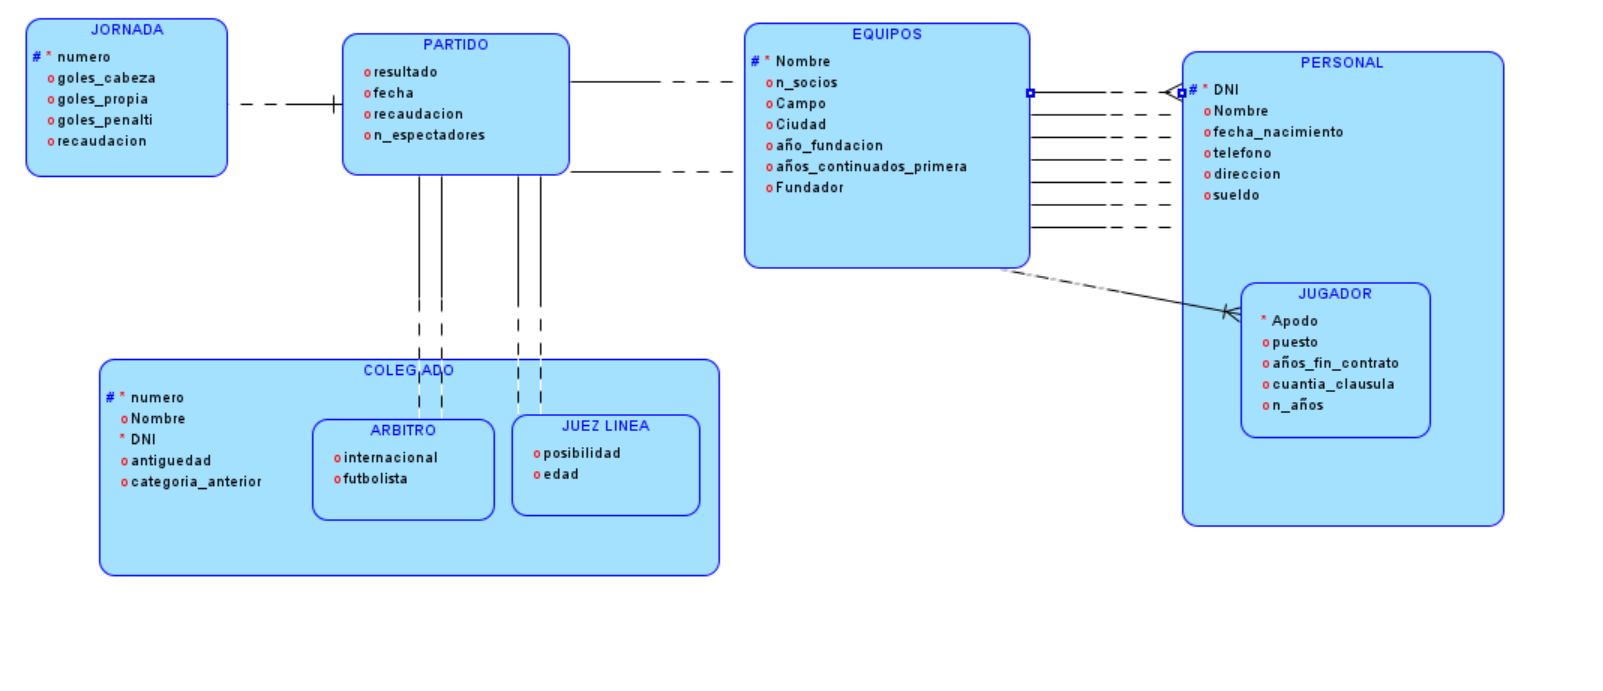
\includegraphics[width=\textwidth]{images/diagrama_logico_futbol.png}
	\caption{Diagrama Lógico De La Liga de Fútbol}
	\label{fig:f_logico}
\end{figure}

\newpage

\subsection{Diseño Entidad Relación}
Una vez acabado el diseño lógico, pasamos a la entidad relación. En este se muestran las claves migrantes que pasarán a otras entidades debido a las relaciones entre ellas (Figura \ref{fig:f_relacional}), como por ejemplo los DNIs heredados por equipo debido a sus múltiples relaciones con personal, o la clave foránea de jugadores (DNI de nuevo) heredada de su supertipo, al igual que lo hacen los subtipos de colegiado. En esta sección podemos observar que se ha creado un nuevo atributo en colegiado llamado COLEGIADO TYPE que indicará si se trata de un árbitro o de un juez de línea. Tenemos también en partido los IDs de los jueces y árbitros que participarán en él y el número de jornada al que corresponde. Jugador indicará además el nombre del equipo al que pertenece.
\\

Los consejeros al ser relación 1:N guardarán información sobre el equipo al que pertenecen dentro de personal.
\\

\begin{figure}[H]
	\centering
	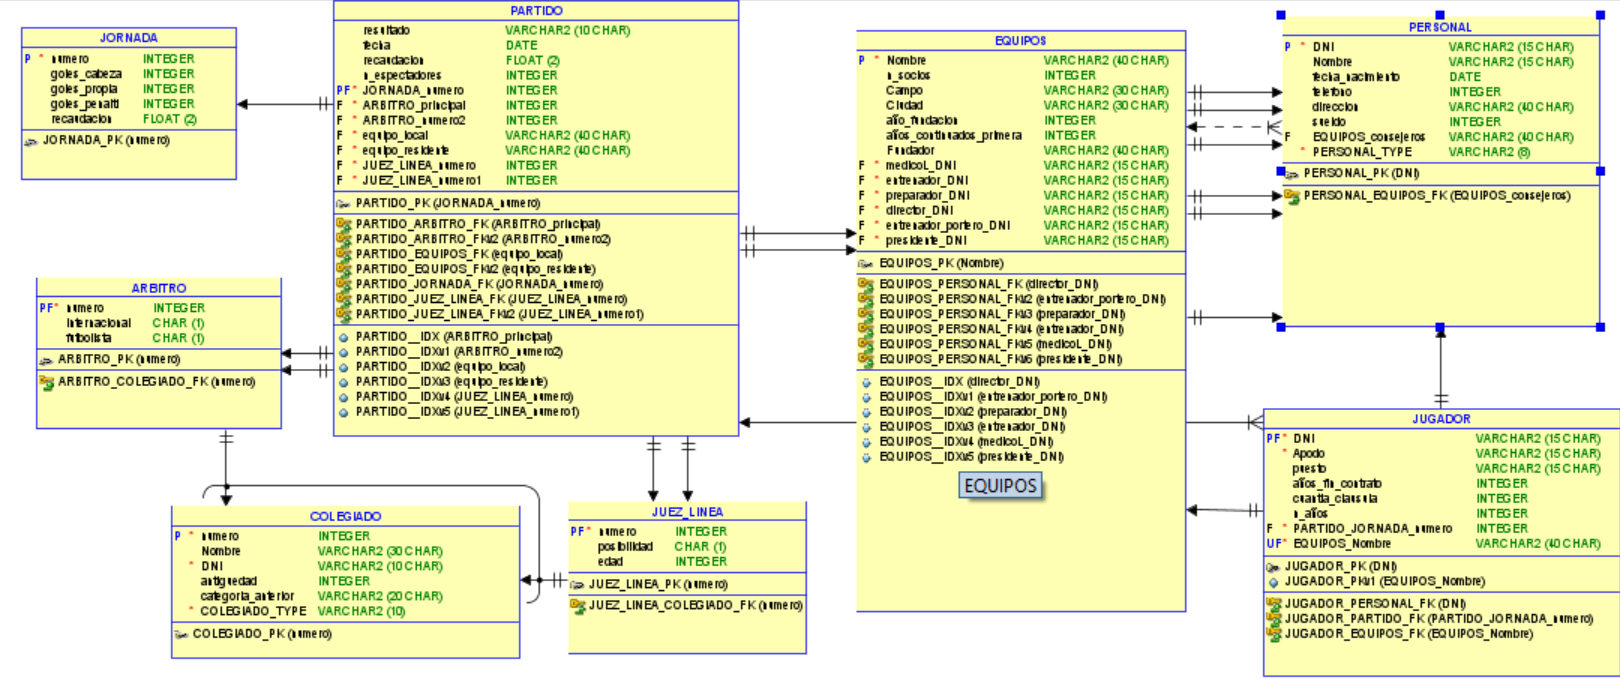
\includegraphics[width=\textwidth]{images/diagrama_relacional_futbol.png}
	\caption{Diagrama Relacional De La Liga de Fútbol}
	\label{fig:f_relacional}
\end{figure}

\newpage
\subsection{Implementación}

En la implementación de la base de datos generaremos el ddl (data definition languaje) e insertaremos tuplas en la misma. En el listing \ref{fig:f_ddl} encontramos una pequeña parte del mismo donde se crea la tabla equipos con sus claves de las relaciones. Esto se ejecutará en Microsoft SQL Server \cite{sqlserver2022} donde se alojará la base de datos.
\begin{lstlisting}[style=ddlstyle, label=fig:f_ddl,caption=Definicion De Datos De La Liga de Fútbol]
	
	CREATE TABLE EQUIPOS 
	(
	Nombre VARCHAR (40) NOT NULL , 
	n_socios INTEGER , 
	Campo VARCHAR (30) , 
	Ciudad VARCHAR (30) , 
	año_fundacion INTEGER , 
	años_continuados_primera INTEGER , 
	Fundador VARCHAR (40) , 
	medicoL_DNI VARCHAR (15) NOT NULL , 
	entrenador_DNI VARCHAR (15) NOT NULL , 
	preparador_DNI VARCHAR (15) NOT NULL , 
	director_DNI VARCHAR (15) NOT NULL , 
	entrenador_portero_DNI VARCHAR (15) NOT NULL , 
	presidente_DNI VARCHAR (15) NOT NULL 
	)
	GO 
	
	CREATE UNIQUE NONCLUSTERED INDEX 
	EQUIPOS__IDX ON EQUIPOS 
	( 
	director_DNI 
	) 
	GO 
	
	CREATE UNIQUE NONCLUSTERED INDEX 
	EQUIPOS__IDXv1 ON EQUIPOS 
	( 
	entrenador_portero_DNI 
	) 
	GO 	
	
	CREATE UNIQUE NONCLUSTERED INDEX 
	EQUIPOS__IDXv2 ON EQUIPOS 
	( 
	preparador_DNI 
	) 
	GO 
	
	CREATE UNIQUE NONCLUSTERED INDEX 
	EQUIPOS__IDXv3 ON EQUIPOS 
	( 
	entrenador_DNI 
	) 
	GO 
	
	CREATE UNIQUE NONCLUSTERED INDEX 
	EQUIPOS__IDXv4 ON EQUIPOS 
	( 
	medicoL_DNI 
	) 
	GO 
		
	CREATE UNIQUE NONCLUSTERED INDEX 
	EQUIPOS__IDXv5 ON EQUIPOS 
	( 
	presidente_DNI 
	) 
	GO
	
	ALTER TABLE EQUIPOS ADD CONSTRAINT EQUIPOS_PK PRIMARY KEY CLUSTERED (Nombre)
	WITH (
	ALLOW_PAGE_LOCKS = ON , 
	ALLOW_ROW_LOCKS = ON )
	GO
	
\end{lstlisting}
	
En el listing \ref{fig:f_insert} se observan ejemplos de las inserciones que se hacen sobre la base de datos, siguiendo un orden lógico para la correcta inserción teniendo en cuenta ciertas dependencias.
\\
\begin{lstlisting}[style=sqlstyle, label=fig:f_insert,caption=Carga de datos]
	-- Insercion de colegiados (incluyendo jueces de línea)
	INSERT INTO COLEGIADO (numero, Nombre, DNI, antiguedad, categoria_anterior, COLEGIADO_TYPE) 
	VALUES 
	(1, 'Antonio Mateu', '12345678A', 10, 'Segunda División', 'ARBITRO'),
	(2, 'Carlos del Cerro', '23456789B', 12, 'Segunda División B', 'ARBITRO'),
	(3, 'José Luis Munuera', '34567890C', 8, 'Segunda División', 'ARBITRO'),
	(4, 'Alejandro Hernández', '45678901D', 9, 'Segunda División', 'ARBITRO'),
	(5, 'Jesús Gil Manzano', '56789012E', 11, 'Segunda División', 'ARBITRO'),
	(6, 'Luis Martínez', '67890123F', 7, 'Segunda División', 'JUEZ_LINEA'),  
	(7, 'Javier López', '78901234G', 6, 'Segunda División', 'JUEZ_LINEA'),  
	(8, 'Fernando Díaz', '89012345H', 5, 'Segunda División', 'JUEZ_LINEA');  
	
	-- Inserción de arbitros
	INSERT INTO ARBITRO (numero, internacional, futbolista) 
	VALUES 
	(1, 1, 0),
	(2, 0, 0),
	(3, 1, 0),
	(4, 0, 1),
	(5, 1, 0);
\end{lstlisting}

\newpage
A continuación se muestra en el listing \ref{fig:f_jugador} una alteración de la tabla jugador previa a la inserción de los datos, debido a una restricción que prohibía que dos jugadores pertenecieran a un mismo equipo.
\\

\begin{lstlisting}[style=sqlstyle, label=fig:f_jugador,caption=Corrección de restricción]
	ALTER TABLE JUGADOR
	DROP CONSTRAINT JUGADOR_PKv1;
	
	-- Insercion de jugadores
	INSERT INTO JUGADOR (DNI, Apodo, puesto, años_fin_contrato, cuantia_clausula, n_años, PARTIDO_JORNADA_numero, EQUIPOS_Nombre) 
	VALUES 
	('DNI1001', 'Benzema', 'Delantero', 2025, 100000000, 5, 1, 'Real Madrid'),
	('DNI1002', 'Modric', 'Centrocampista', 2024, 50000000, 8, 1, 'Real Madrid'),
	('DNI1003', 'Ter Stegen', 'Portero', 2026, 80000000, 5, 2, 'FC Barcelona'),
	('DNI1004', 'Pedri', 'Centrocampista', 2026, 150000000, 6, 2, 'FC Barcelona'),
	('DNI1005', 'Koke', 'Centrocampista', 2025, 60000000, 4, 3, 'Atletico Madrid'),
	('DNI1006', 'Navas', 'Defensa', 2024, 30000000, 3, 4, 'Sevilla FC');
	
\end{lstlisting}

\newpage
\subsection{Consultas}
Una vez implementados correctamente todos los datos y rellenadas las tablas, procedemos a la realización de consultas (listing \ref{fig:f_consultas}).
\\


\begin{lstlisting}[style=sqlstyle, label=fig:f_consultas,caption=Consultas Sobre La Liga de Fútbol]
	
	--CONSULTA 1: Salario medio de los entrenadores de los equipos
	SELECT AVG(p.sueldo) as salario_medio_entrenadores
	FROM EQUIPOS e, PERSONAL p 
	WHERE e.entrenador_DNI = p.dni;
	
	--CONSULTA 2: Nombre, antiguedad y tipo de los colegiados con mas de 6 años de antiguedad
	SELECT Nombre,antiguedad, COLEGIADO_TYPE
	FROM COLEGIADO
	WHERE antiguedad>6
	ORDER BY antiguedad;
	
	--CONSULTA 3: Muestra el nombre de los arbitros que han participado en al menos dos partidos y que son internacionales
	SELECT distinct( c.Nombre)
	FROM COLEGIADO c
	JOIN ARBITRO a ON c.numero = a.numero
	JOIN PARTIDO p ON p.ARBITRO_principal = c.numero OR p.ARBITRO_numero2 = c.numero
	WHERE a.internacional = 1
	GROUP BY c.Nombre
	HAVING COUNT(c.numero) >= 2;
	
	--CONSULTA 4: Muestra los goles totales de cada jornadas
	SELECT numero, SUM(goles_cabeza + goles_propia + goles_penalti) as total_goles
	FROM JORNADA
	GROUP BY numero;
	
	--CONSULTA 5: Recaudacion media por espectador en cada partido
	SELECT equipo_local, equipo_residente, recaudacion/n_espectadores as recaudacion_media
	FROM PARTIDO;
	
\end{lstlisting}
	
\newpage
\section{Acceso al Repositorio}

Toda la información adicional, incluyendo el código fuente y la documentación completa de este proyecto, está disponible en el repositorio de GitHub \cite{silva2024github}.

% Incluir la bibliografía
\bibliographystyle{plain}  % Estilo de la bibliografía (por ejemplo, plain, alpha, ieee, etc.)
\bibliography{bibli}  % Nombre del archivo .bib sin la extensión

\end{document}
